% !TEX TS-program = pdflatex
% !TEX encoding = UTF-8 Unicode

% This is a simple template for a LaTeX document using the "article" class.
% See "book", "report", "letter" for other types of document.

\documentclass{article} % use larger type; default would be 10pt

\usepackage[utf8]{inputenc} % set input encoding (not needed with XeLaTeX)

%%% Examples of Article customizations
% These packages are optional, depending whether you want the features they provide.
% See the LaTeX Companion or other references for full information.

%%% PAGE DIMENSIONS
\usepackage{geometry} % to change the page dimensions
\geometry{a4paper} % or letterpaper (US) or a5paper or....
 \geometry{margin=3cm} % for example, change the margins to 2 inches all round
% \geometry{landscape} % set up the page for landscape
%   read geometry.pdf for detailed page layout information

\usepackage{graphicx} % support the \includegraphics command and options

% \usepackage[parfill]{parskip} % Activate to begin paragraphs with an empty line rather than an indent

%%% PACKAGES
%\usepackage{booktabs} % for much better looking tables
%\usepackage{array} % for better arrays (eg matrices) in maths
%\usepackage{paralist} % very flexible & customisable lists (eg. enumerate/itemize, etc.)
%\usepackage{verbatim} % adds environment for commenting out blocks of text & for better verbatim
%\usepackage{subfig} % make it possible to include more than one captioned figure/table in a single float
% These packages are all incorporated in the memoir class to one degree or another...
\usepackage{tikz}
\usetikzlibrary{shapes,arrows,matrix,decorations.pathreplacing,automata,arrows.meta}

%%% HEADERS & FOOTERS
%\usepackage{fancyhdr} % This should be set AFTER setting up the page geometry
%\pagestyle{fancy} % options: empty , plain , fancy
%\renewcommand{\headrulewidth}{0pt} % customise the layout...
%\lhead{}\chead{}\rhead{}
%\lfoot{}\cfoot{\thepage}\rfoot{}

%%% SECTION TITLE APPEARANCE
%\usepackage{sectsty}
%\allsectionsfont{\sffamily\mdseries\upshape} % (See the fntguide.pdf for font help)
% (This matches ConTeXt defaults)

%%% ToC (table of contents) APPEARANCE
%\usepackage[nottoc,notlof,notlot]{tocbibind} % Put the bibliography in the ToC
%\usepackage[titles,subfigure]{tocloft} % Alter the style of the Table of Contents
%\renewcommand{\cftsecfont}{\rmfamily\mdseries\upshape}
%\renewcommand{\cftsecpagefont}{\rmfamily\mdseries\upshape} % No bold!

%%% END Article customizations

%%% The "real" document content comes below...

\title{Hierarchy of Extended Finite-State Machines}
\author{Michal Soucha}
%\date{8. 8. 2017}

\newcommand{\reward}{\textcolor{orange}{0}}
\newcommand{\rewardPos}{\textcolor{green!50!black}{1}}
\newcommand{\rewardNeg}{\textcolor{red}{-1}}
\newcommand{\guard}[1]{~if \textcolor{magenta}{#1}}
\newcommand{\action}[1]{~~\textcolor{blue}{#1}}

\begin{document}
\maketitle

\section{Why use extended finite-state machines?}

{\em Extended finite-state machines} (EFSM) are powerful abstract models of any system
that can be described by a {\em regular language}.
As all tasks of the General AI Challenge are regular languages,
EFSMs can represent the tasks accurately and so provide correct outputs.
The main advantage over other representations is that
 EFSMs are {\bf easy to understand and analyse} for both people and computers,
 see the examples of EFSMs in Figure~\ref{efsm} on page 3.

An EFSM consists of finite number of states, transitions between them, and structures holding data.
As only the deterministic behaviour is considered, the modelled system is always in exactly one state
called the current state.
The current state is changed according to inputs applied to the system and corresponding transitions.
Each transition is labelled with an {\em input} symbol, an {\em output} symbol, a {\em reward}, 
a {\em guard} and an {\em action} such that
the guard is a condition that needs to be satisfied to follow the transition,
and the action can change the data structures. 
The guard and the action can be missing on a transition as can be seen in Figure~\ref{efsm}.
There can be several transition with the same input from a state but
then the outputs, the rewards, or the guards need to distinguish the transitions
so that at most one transition corresponds to the applied input and the observed output and reward.
This secures that the system cannot be in several states at once.
On the other hand, there can be no suitable transition from the current state,
then the model does not describe the system. 
For example, when the task is changed, the model of the previous task does not represent the new task.
EFSMs without the data structures and guards and actions on transitions are called
{\em observable deterministic finite-state machines} (ODFSM) and they are accurate
to model the traces, that is, the observed sequences of input-output-reward tuples.

\section{Learning EFSM hierarchy}

EFSMs modelling the tasks of Challenge contains just one cycle of transitions that start and ends in the initial state.
The cycle correspond to one run of a task instance.
This important property allows one to establish a hierarchy of EFSMs
with a tree representation such that children are specializations of their parent.
The root of hierarchy is an EFSM with just the initial state and requires an output on any applied input
such that the reward can be arbitrary.
Its child, a specialized model, can be for example an 1-state EFSM prescribing a particular output for all inputs (Micro-task 1).
The root is thus a generalization of all other EFSMs in the hierarchy. 
Part of the hierarchy is captured in Figure~\ref{efsm}.

Learning a new EFSMs, and so solving a task, has three phases as follows.

\begin{enumerate}
\item {\em Specialization} of the conjectured model -- the conjectured model is initialized
with the model of hierarchy that is consistent with the current trace but no its child is and
 it was used correctly the most amongst such models.
Its specialization with the ODFSM covering the current trace finds common control pattern in the task instance
like there is a command name followed by a colon (Micro-task 6 and up) or there is a period after the feedback.
\item {\em Learning a data pattern} -- specialization stripped the control flow so data parts can be easily analysed
and for example `interleaving' pattern can be found. 
If no pattern found, a mapping of input to output mentioned in feedback is used.
\item {\em Generalization} of the learned model -- the conjectured model is stored to the hierarchy after
the task instance is changed (it fails to provide accurate outputs and at least 5 consecutive positive rewards were recorded).
It is tried to generalize itself and then with its siblings (models in the hierarchy with the same parent) such that
the generalized model is a specialization of their parent. 
The aim is to have a more accurate `initial' model for next tasks.
Finally, the current trace and related ODFSM is cleared and the phase 1 starts for the new task instance.
If the conjectured model fails but the task instance was not learnt, 
then the phase 1 starts again after throwing the incorrect conjectured model away.
\end{enumerate}

Having models of all learnt tasks with their generalized versions is beneficial 
because one can analyse and combine them and so
next related task can be solved faster.

\section{Prototype of the Gradual EFSM Learner}

A prototype of the EFSM learner was implemented in Python.
It does not cover the entire idea so it is rather a showcase how efficient the learning
using EFSM hierarchy can be.
I focused on the learning of commands so the first four Micro-tasks were skipped.
The `basic communication' EFSM shown in the middle of Figure~\ref{efsm}
is considered as the root of hierarchy.
The model is possible to learn from the Micro-tasks 1--5 with an implementation of full idea
(that would take me more than spare time of one month).

In the current implementation, each EFSM has two data structures, $words$ and $mapping$, and two variables, $output$ and $y$.
As the implemented phase 2 can detect only simple patterns like copying, interleaving and reverse order,
the Learner solves the Micro-tasks 5.3--9 but should be able to learn even the Micro-tasks 14 and 15 easily.
The phase 2 could use neural nets or a pool of function that the Learner could combine. That is a future work.

The Learner accepts two file names as optional arguments. The first is name of a pickled prelearned hierarchy;
if the empty string is given, the Learner starts with just the basic communication EFSM as the root.
The hierarchy is stored to `brainTmp.pkl' after each task instance is learnt.
If the second argument is provided, the Learner stores the hierarchy in the DOT language to the file with the given name.
The hierarchy can be then visualized in FSMvis (based on visjs.org) that is submitted with the source codes.

\section{Conclusion}

Learning EFSM hierarchy is suitable to use when regular languages are to learn
as the hierarchy provides {\bf accurate models} that are {\bf understandable for people}
so that one knows exactly how the machine `thinks'.

\begin{figure}[h]
\begin{center}
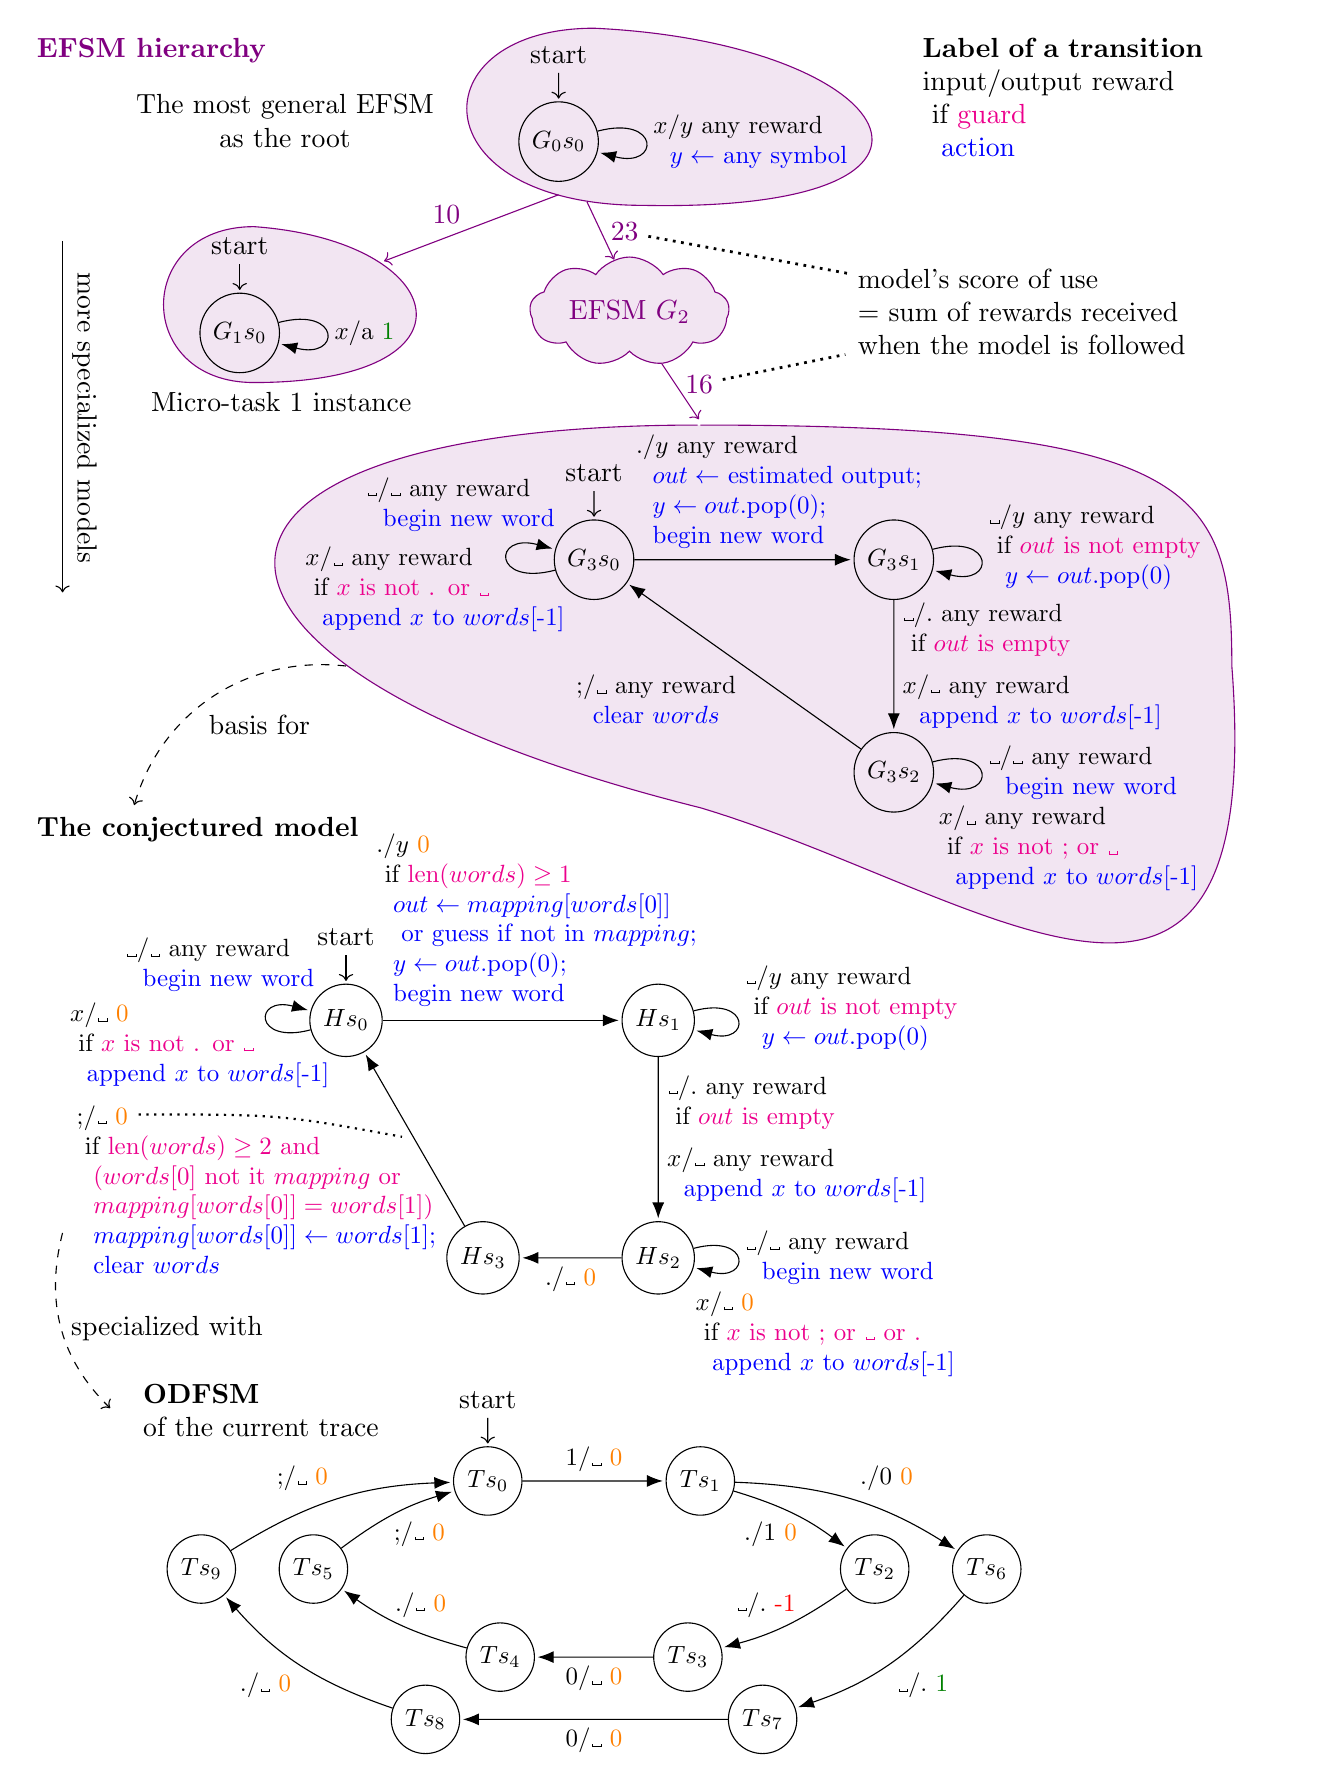
\begin{tikzpicture}[scale=0.9,shorten >=1pt]
\tikzstyle{every state}=[scale=0.9,node distance=3cm]
\tikzstyle{initialState}=[state,initial above,initial distance=4mm,-{Latex[scale=0.9]}]
\tikzstyle{edgeLabel}=[scale=0.9,auto]
\tikzstyle{efsm}=[draw,violet,fill=violet!10!white]
\path[efsm] 
(3.5,14) .. controls (7.8,13.8) and (9.3,11.4) .. (4.2,11.5) .. controls (1,11.5) and (1,14) .. (3.5,14)
(-1.3,11.2) .. controls (1.5,11) and (2,9) .. (-1.3,9) .. controls (-3,9) and (-3,11.2) .. (-1.3,11.2)
(5,8.4) .. controls (12,8.4) and (12.5,7.5) .. (12.5,5) .. controls (13,-1.5) and (9,1.8) .. (5,3) 
.. controls (-3,5) and (-3,8.4) .. (5,8.4)
;
\draw[violet] 
(3,11.65) edge [->] node[left,yshift=5] {10} (0.5,10.7)
(3.4,11.55) edge [->] node[right] (rew1) {23} (3.8,10.7)
(4.3,9.5) edge [->] node[right] (rew2) {16} (5,8.45)
;
\draw node[text width=5cm] (score) at (10,10) {model's score of use\\= sum of rewards received\\ when the model is followed}
[dotted,line width=1pt]
(rew1) -- (score)
(rew2) -- (score)
;
\path node[anchor=north west] at(-4.5,14) {\bf\textcolor{violet}{EFSM hierarchy}}
node[anchor=north west,text width=45mm,text centered] at(-3.5,13.2) {The most general EFSM\\ as the root}
(-4,11) edge [draw,->] node[midway,above,sloped] {more specialized models} (-4,6)

node[text width=40mm,anchor=north west] at (8,14) {{\bf Label of a transition}\\input/output~reward\\
\guard{guard}\\
\action{action}}

node[initialState] (G0s0) at (3,12.4) {$G_0 s_0$}

node[initialState] (Gis0) at (-1.5,9.7) {$G_1 s_0$}
node[yshift=-25,xshift=15] at (Gis0) {Micro-task 1 instance}

node[cloud,draw,cloud puffs=9,cloud puff arc=110,aspect=2.5,inner ysep=0em,efsm] at (4,10) {EFSM $G_2$}

node[initialState] (G1s0) at (3.5,6.5) {$G_3 s_0$}
node[state,xshift=35] (G1s1) [right of=G1s0] {$G_3 s_1$}
node[state] (G1s2) [below of=G1s1] {$G_3 s_2$}

(0,5) edge [->,draw,dashed,bend right=40] node[right,xshift=-5,yshift=-10] {basis for} (-3,3)
node[anchor=north west] at (-4.5,3) {\bf The conjectured model}
node[initialState] (G2s0) at (0,0) {$H s_0$}
node[state,xshift=40] (G2s1) [right of=G2s0] {$H s_1$}
node[state,yshift=-10] (G2s2) [below of=G2s1] {$H s_2$}
node[state,xshift=15] (G2s3) [left of=G2s2] {$H s_3$}

node[anchor=north west,text width=5cm] at (-3,-5) {{\bf ODFSM}\\ of the current trace}
(-4,-3) edge [->,draw,dashed,bend right] node[right] {specialized with} (-3.3,-5.5)
node[initialState] (G3s0) at (2,-6.5) {$T s_0$}
node[state] (G3s1) [right of=G3s0] {$T s_1$}
node[state,xshift=70,yshift=50] (G3s2) [below of=G3s1] {$T s_2$}
node[state,xshift=-70,yshift=50] (G3s5) [below of=G3s0] {$T s_5$}
node[state,xshift=-75,yshift=50] (G3s3) [below of=G3s2] {$T s_3$}
node[state,xshift=75,yshift=50] (G3s4) [below of=G3s5] {$T s_4$}
node[state,xshift=45] (G3s6) at (G3s2) {$T s_6$}
node[state,xshift=30,yshift=-25] (G3s7) at (G3s3) {$T s_7$}
node[state,xshift=-30,yshift=-25] (G3s8) at (G3s4) {$T s_8$}
node[state,xshift=-45] (G3s9) at (G3s5) {$T s_9$}
;
\path [->,>={Latex[scale=1.2]},shorten >=1pt] 
(G0s0) edge [loop right] node[edgeLabel,text width=40mm] {$x$/$y$ any reward\\\action{$y\gets$ any symbol}} ()

(Gis0) edge [loop right] node[edgeLabel,text width=40mm] {$x$/a \rewardPos} ()

(G1s0) edge [loop left] node[edgeLabel,text width=40mm,above,xshift=0,yshift=8] {
\textvisiblespace/\textvisiblespace~any reward\\
\action{begin new word}}
node[edgeLabel,text width=40mm,xshift=36,yshift=-12] {$x$/\textvisiblespace~any reward\\
\guard{$x$ is not . or \textvisiblespace}\\
\action{append $x$ to $words$[-1]}} ()
(G1s0) edge node[edgeLabel,text width=41mm,xshift=15,yshift=1] {./$y$~any reward\\
\action{$out \gets$ estimated output;}\\\action{$y\gets out$.pop(0);}\\\action{begin new word}} (G1s1)
(G1s1) edge [loop right] node[edgeLabel,text width=4cm,yshift=5] {\textvisiblespace/$y$~any reward\\
\guard{$out$ is not empty}\\
\action{$y\gets out$.pop(0)}} ()
(G1s1) edge node[edgeLabel,text width=4cm] {\textvisiblespace/.~any reward\\\guard{$out$ is empty}\\[5pt]
$x$/\textvisiblespace~any reward\\\action{append $x$ to $words$[-1]}} (G1s2)
(G1s2) edge [loop right] node[edgeLabel,text width=45mm] {\textvisiblespace/\textvisiblespace~any reward\\
\action{begin new word}}
node[edgeLabel,text width=45mm,below right,yshift=-10,xshift=-20] {$x$/\textvisiblespace~any reward\\
\guard{$x$ is not ; or \textvisiblespace}\\
\action{append $x$ to $words$[-1]}} ()
(G1s2) edge node[edgeLabel,text width=4cm,xshift=50] {;/\textvisiblespace~any reward\\
\action{clear $words$}} (G1s0)

(G2s0) edge [loop left] node[edgeLabel,text width=40mm,above,xshift=0,yshift=8] {
\textvisiblespace/\textvisiblespace~any reward\\
\action{begin new word}}
 node[edgeLabel,text width=40mm,xshift=38,yshift=-10] {$x$/\textvisiblespace~\reward\\
\guard{$x$ is not . or \textvisiblespace}\\
\action{append $x$ to $words$[-1]}} ()
(G2s0) edge node[edgeLabel,text width=46mm,xshift=15,yshift=2] {./$y$~\reward\\
\guard{len($words) \ge 1$}\\
\action{$out \gets mapping[words[0]]$}\\\action{~or guess if not in $mapping$;}
\\\action{$y\gets out$.pop(0);}\\\action{begin new word}} (G2s1)
(G2s1) edge [loop right] node[edgeLabel,text width=4cm,yshift=5] {\textvisiblespace/$y$~any reward\\
\guard{$out$ is not empty}\\
\action{$y\gets out$.pop(0)}} ()
(G2s1) edge node[edgeLabel,text width=4cm] {\textvisiblespace/.~any reward\\\guard{$out$ is empty}\\[5pt]
$x$/\textvisiblespace~any reward\\\action{append $x$ to $words$[-1]}} (G2s2)
(G2s2) edge [loop right] node[edgeLabel,text width=45mm] {\textvisiblespace/\textvisiblespace~any reward\\
\action{begin new word}}
node[edgeLabel,text width=45mm,below right,yshift=-10,xshift=-20] {$x$/\textvisiblespace~\reward\\
\guard{$x$ is not ; or \textvisiblespace~or .}\\
\action{append $x$ to $words$[-1]}} ()
(G2s2) edge node[edgeLabel] {./\textvisiblespace~\reward} (G2s3)
(G2s3) edge node (G2edge) {}
node[edgeLabel,text width=51mm,xshift=13,yshift=17] (G2edgeLabel) {;/\textvisiblespace~\reward\\
\guard{len($words) \ge 2$ and\\
~~($words[0]$ not it $mapping$ or\\
~~$mapping[words[0]] = words[1])$}\\
\action{$mapping[words[0]] \gets words[1]$;}\\
\action{clear $words$}} (G2s0)

(G3s0) edge node[edgeLabel] {1/\textvisiblespace~\reward} (G3s1)
(G3s1) edge [bend left=10] node[edgeLabel,left,xshift=5,yshift=-8] {./1~\reward} (G3s2)
(G3s2) edge [bend left=10] node[edgeLabel,left,xshift=7,yshift=8] {\textvisiblespace/.~\rewardNeg} (G3s3)
(G3s3) edge node[edgeLabel] {0/\textvisiblespace~\reward} (G3s4)
(G3s4) edge [bend left=10] node[edgeLabel,right,xshift=-6,yshift=8] {./\textvisiblespace~\reward} (G3s5)
(G3s5) edge [bend left=10] node[edgeLabel,right,xshift=-4,yshift=-8] {;/\textvisiblespace~\reward} (G3s0)
(G3s1) edge [bend left=15] node[edgeLabel] {./0~\reward} (G3s6)
(G3s6) edge [bend left=15] node[edgeLabel] {\textvisiblespace/.~\rewardPos} (G3s7)
(G3s7) edge node[edgeLabel] {0/\textvisiblespace~\reward} (G3s8)
(G3s8) edge [bend left=15] node[edgeLabel] {./\textvisiblespace~\reward} (G3s9)
(G3s9) edge [bend left=15] node[edgeLabel] {;/\textvisiblespace~\reward} (G3s0)
;
\draw[dotted,line width=0.8pt] (G2edgeLabel.north west) +(1,-.25) ..controls +(2,0) ..  (G2edge);
%(L) edge [loop left] node[edgeLabel,below,yshift=-12,xshift=12] {p/\textcolor{red}{L}} ()
%(L) edge [bend left] node[edgeLabel] {c/\textcolor{blue}{N}} (U)
%(U) edge [loop right] node[edgeLabel,below,yshift=-12,xshift=-12] {c/\textcolor{blue}{N}} ()
%(U) edge [bend left] node[edgeLabel] {p/\textcolor{green!50!black}{F}} (L);
\end{tikzpicture}\end{center}
\caption[EFSM hierarchy]
{A part of the EFSM hierarchy during learning the Micro-task 5.5}\label{efsm}
\end{figure}

\end{document}
